\documentclass[../norme-di-progetto.tex]{subfiles}
\begin{document}
\subsection{Fornitura}
\subsubsection{Scopo}
Lo scopo di questo processo consiste nel:
\begin{itemize}
  \item Determinare le competenze e gli strumenti necessari per lo svolgimento del progetto; questo viene documentato nello \textsc{Studio di Fattibilità};
  \item Descrivere l'organizzazione del lavoro che porterà il gruppo alla realizzazione del prodotto del capitolato scelto; questo viene fatto nel \textsc{Piano di Progetto};
  \item Stabilire se il materiale prodotto soddisfa ben definiti obiettivi di qualità; questi sono definiti nel \textsc{Piano di Qualifica}.
\end{itemize}
Il processo di fornitura è composto dalle seguenti fasi:
\begin{itemize}
  \item Avvio;
  \item Preparazione di risposte alle richieste;
  \item Contrattazione;
  \item Pianificazione;
  \item Esecuzione e controllo;
  \item Revisione e valutazione;
  \item Consegna e completamento.
\end{itemize}
\subsubsection{Aspettative}
L'aspettativa di questo processo è quella di mantenere un confronto frequente con il proponente per:
\begin{itemize}
  \item Determinare i requisiti del prodotto da lui desiderato;
  \item Stimare le tempistiche di lavoro;
  \item Avere una verifica continua di quanto prodotto;
  \item Chiarire eventuali dubbi.
\end{itemize}
\subsubsection{Descrizione}
In questa sezione vengono descritti i documenti precedentemente citati.
\subsubsection{Attività}
\paragraph{Studio di fattibilità}
Lo \textsc{Studio di Fattibilità}, redatto dagli Analisti, fornisce una breve descrizione di tutti i capitolati proposti. Per ogni capitolato viene indicato:
\begin{itemize}
  \item \textbf{Informazioni generali}: le informazioni di base del capitolato, comprendenti il nome, il proponente e il committente;
  \item \textbf{Descrizione}: una breve presentazione che introduce le caratteristiche principali del capitolato;
  \item \textbf{Finalità del progetto}: una descrizione dettagliata degli obiettivi e della finalità del prodotto che il capitolato chiede di sviluppare;
  \item \textbf{Tecnologie interessate}: le tecnologie interessate dal progetto, comprendente i linguaggi di programmazione e gli strumenti che il gruppo dovrà utilizzare per lo sviluppo;
  \item \textbf{Aspetti positivi}: i punti a favore della scelta del capitolato emersi dopo la discussione tra i componenti del gruppo;
  \item \textbf{Rischi}: le criticità e gli eventuali rischi da fronteggiare in caso di scelta del capitolato;
  \item \textbf{Conclusione}: le ragioni per le quali il gruppo ha deciso di accettare o non accettare il capitolato.
\end{itemize}
\paragraph{Piano di Progetto}
Il \textsc{Piano di Progetto}, redatto dal Responsabile, contiene:
\begin{itemize}
  \item %%% IN ATTESA DEL PdP
\end{itemize}
\paragraph{Piano di Qualifica}
Il \textsc{Piano di Qualifica}, redatto dai Verificatori, contiene le strategie, le linee guida e i processi che il gruppo deve adottare al fine di garantire lo sviluppo un prodotto di qualità. In aggiunta a questo, esso contiene le norme che regolano la \glossario{qualità di processo}, le quali assicurano che i membri del gruppo lavorino secondo le metriche scelte. \\
Questo documento contiene le seguenti sezioni chiave:
\begin{itemize}
  \item \textbf{Qualità di processo}: sono qui identificati dei processi, scelti dagli standard, stabiliti degli obiettivi, ideate delle strategie per attuarli e, infine, individuate e documentate le metriche per misurarli;
  \item \textbf{Qualità di prodotto}: sono qui identificati gli obiettivi per raggiungere le caratteristiche più rilevanti per il prodotto, e le metriche per misurarli;
  %%% QUESTO È DA AGGIUNGERE NEL PdQ %%%
  \item \textbf{Specifiche dei test}: è qui definito un insieme di test a cui sottoporre il prodotto per garantire il soddisfacimento dei requisiti;
  \item \textbf{Standard di qualità}: vengono qui elencati e descritti gli standard ISO di qualità scelti dal gruppo;
  \item \textbf{Resoconto attività di verifica}: vengono qui resi noti i risultati dei test relativi al periodo di revisione dei documenti e dei requisiti, ottenuti mediante l'utilizzo delle metriche esposte nel documento;
  \item \textbf{Valutazioni per il miglioramento}: questa sezione elenca i problemi riscontrati nel corso del progetto.
\end{itemize}
Il \textsc{Piano di Qualifica} è un documento destinato ad evolversi ed essere modificato durante la durata del progetto, poiché le metriche e i processi identificati inizialmente possono rivelarsi insufficienti o inadatti al mantenimento della qualità.
\paragraph{Strumenti}
Il processo di fornitura viene coadiuvato dall'utilizzo di strumenti software.
\subparagraph{GanttProject}
GanttProject è un software di \textit{project management} che permette di progettare lo \textit{scheduling} di tasks e organizzare le risorse con l'ausilio di grafici. Questo strumento è stato utilizzato principalmente per costruire i diagrammi di Gantt presenti nel \textsc{Piano di Progetto}.

\begin{figure}[H]
  \centering
  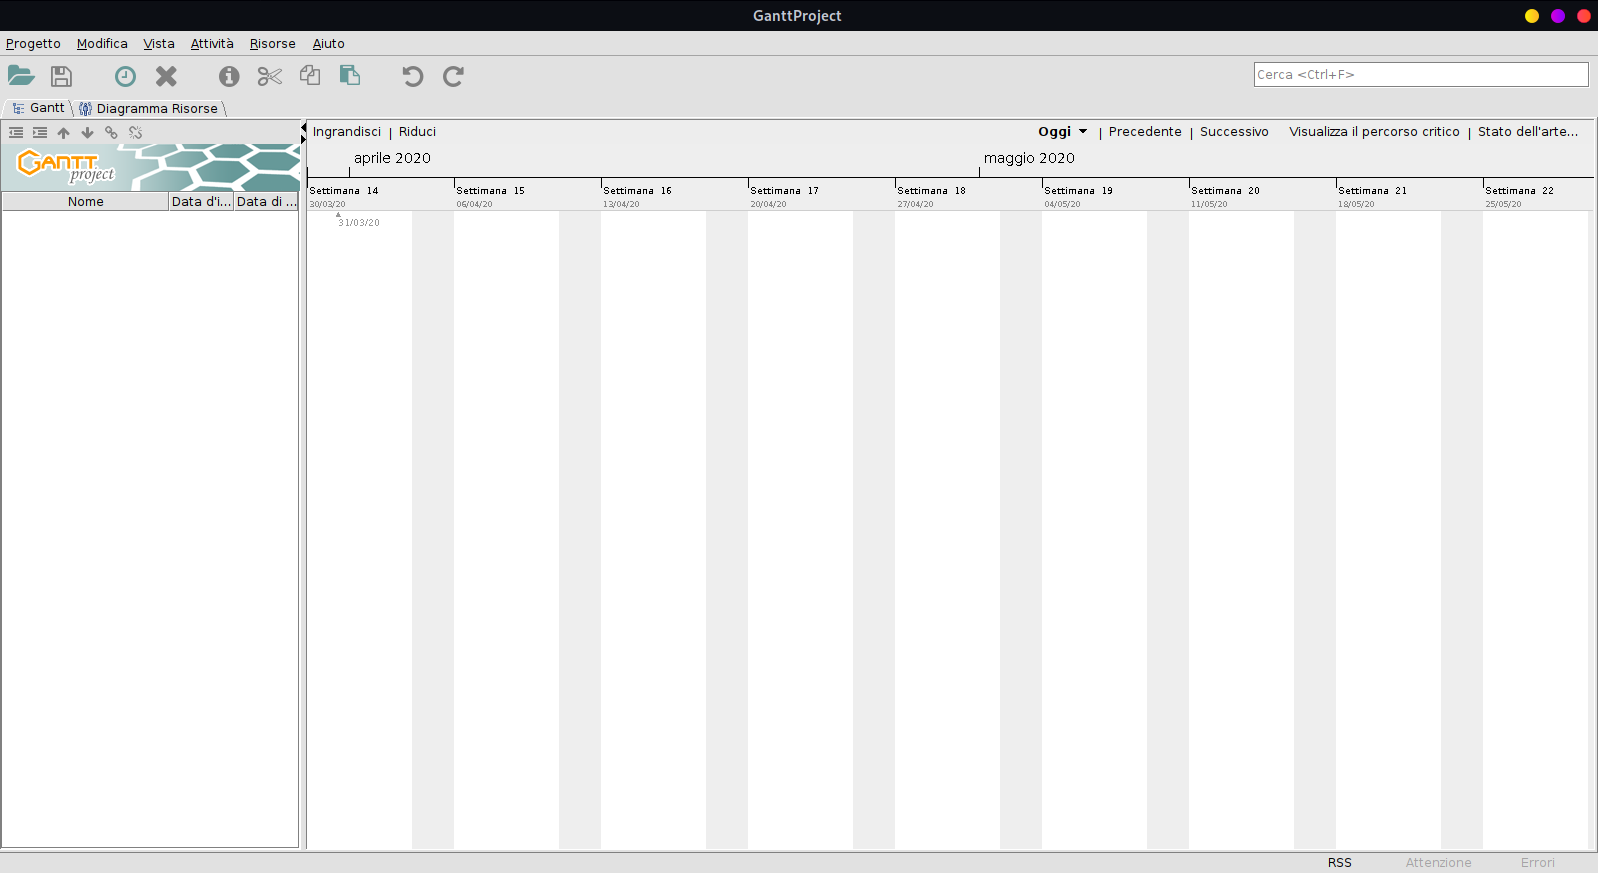
\includegraphics[width=10cm]{img/gantt.png}
  \label{fig:gantt}
  \caption{GanttProject per GNU/Linux.}
\end{figure}

\subparagraph{Google Sheets}
Google Sheets è un programma, appartenente alla \textit{suite office} di Google, per la creazione di fogli di calcolo. Questo applicativo è stato usato dal gruppo per la creazione delle tabelle e dei grafici presenti nel \textsc{Piano di Progetto}.

\begin{figure}[H]
  \centering
  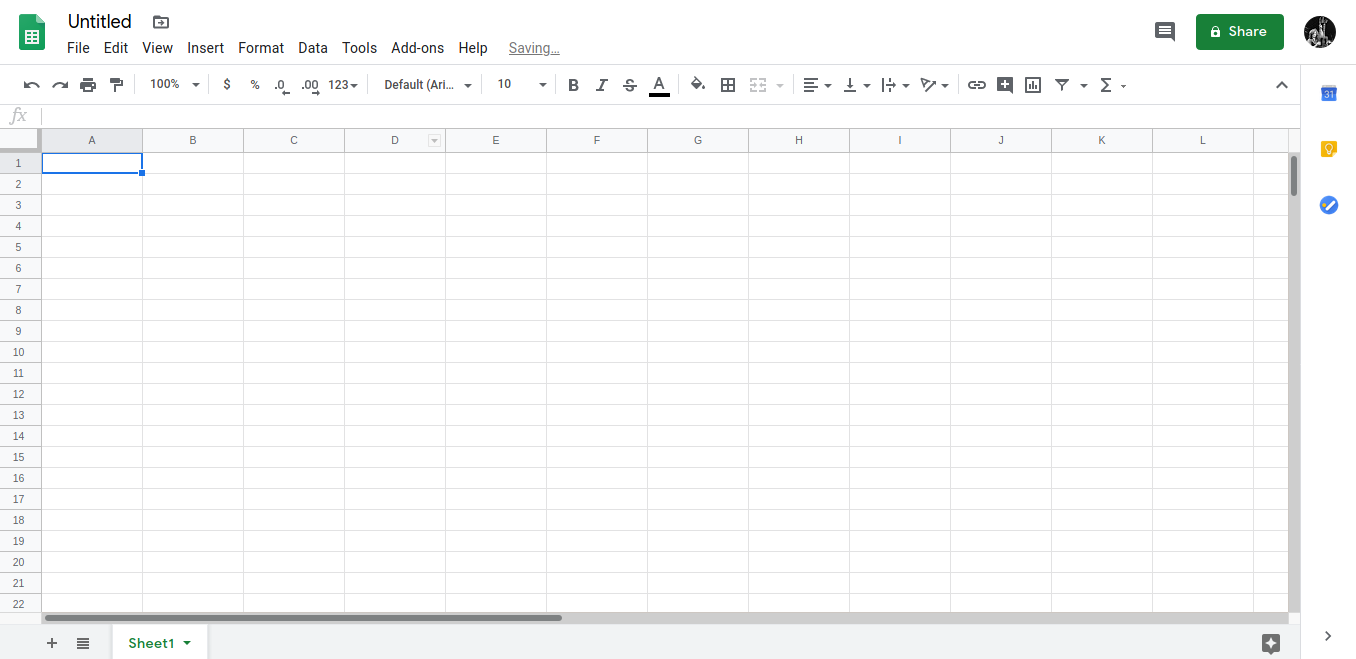
\includegraphics[width=10cm]{img/sheets.png}
  \label{fig:sheets}
  \caption{Piattaforma online \href{https://docs.google.com/spreadsheets/u/0/}{Google Sheets}.}
\end{figure}

\subsection{Sviluppo}
\subsubsection{Scopo}
Lo scopo di questo processo è descrivere le attività e i compiti che il gruppo deve svolgere, al fine di realizzare il prodotto finale richiesto dal proponente.
\subsubsection{Aspettative}
Le aspettative di questo processo sono le seguenti:
\begin{itemize}
  \item Fissare gli obiettivi di sviluppo;
  \item Fissare i vincoli tecnologici e di design;
  \item Realizzare un prodotto finale che:
  \begin{itemize}
    \item Rispetti i requisiti e le richieste del proponente;
    \item Superi i test.
  \end{itemize}
\end{itemize}
\subsubsection{Descrizione}
Il processo di sviluppo si articola nelle seguenti attività:
\begin{itemize}
  \item Analisi dei Requisiti;
  \item Progettazione;
  \item Qualifica.
\end{itemize}
\subsubsection{Attività}
\paragraph{Analisi dei requisiti}
\subparagraph{Scopo}
Lo scopo dell'\textsc{Analisi dei Requisiti}, redatto dagli Analisti, definisce e quindi elenca tutti i requisiti del capitolato. Il documento quindi conterrà:
\begin{itemize}
  \item %%% IN ATTESA DELL'AdR %%%
\end{itemize}
\subparagraph{Aspettative}
L'aspettativa di questo processo coincide con la creazione del documento \textsc{Analisi dei Requisiti}, il quale contiene appunto i requisiti richiesti dal proponente per la realizzazione del progetto.
\subparagraph{Descrizione}
I requisiti sono catalogati secondo un ordine preciso:
\begin{itemize}
  \item %%% IN ATTESA DELL'AdR %%%
\end{itemize}
%%% IN ATTESA DELL'AdR %%%
\subparagraph{Classificazione dei requisiti}
\subparagraph{Classificazione dei casi d'uso}

\paragraph{Progettazione}
\subparagraph{Scopo}
Lo scopo di questa attività è quello di definire le caratteristiche del prodotto richiesto, in funzione dei requisiti elencati nell'\textsc{Analisi dei Requisiti}.
\subparagraph{Aspettative}
L'aspettativa di questa attività coincide con la realizzazione dell'architettura del sistema.
\subparagraph{Descrizione}
%%% IN ATTESA DELL'AdR %%%
\paragraph{Codifica}
\subparagraph{Scopo}
Lo scopo di questa attività è quella di forire le regole per la scrittura del codice Javascript. La codifica coincide con la programmazione stessa del prodotto; è quindi a opera dei Programmatori, i quali dovranno seguire le seguenti regole al fine di ottenere un prodotto coerente e uniforme in tutte le sue componenti.
\subparagraph{Aspettative}
Le aspettative di questo processo sono:
\begin{itemize}
  \item Ottenere un prodotto software conforme ai requisiti concordati con il proponente;
  \item Assicurare l'uniformità di produzione delle diverse componenti del prodotto;
  \item Assicurare che il codice prodotto sia:
  \begin{itemize}
    \item Uniforme nella sua struttura;
    \item Leggibile e di facile comprensione, nell'ottica della futura verifica, validazione e manutenzione del prodotto.
  \end{itemize}
\end{itemize}
\subparagraph{Descrizione}
Il codice dovrà essere scritto rispettando quanto documentato; nello specifico, esso dovrà perseguire gli obiettivi di qualità definiti nel documento \textsc{Piano di Qualifica}.

\subparagraph{Intestazione}
Ogni file contenente codice dovrà possedere la seguente intestazione:
\begin{lstlisting}
 /*
 * File: nome file
 * Version: versione file
 * Date: data creazione
 * Author: nome autore
 * Descrizione: breve descrizione file
 * Appunti: eventuali appunti da fare (avvertenze, dipendenze...)
 */
\end{lstlisting}

\subparagraph{Stile}
Al fine di ottenere una scrittura omogenea e uniforme del codice, ogni membro del gruppo è tenuto a rispettare le seguenti norme:
\begin{itemize}
  \item \textbf{Nomi delle funzioni e delle variabili}: le funzioni e le variabili locali seguono la codifica \glossario{camelCase}:
      \begin{itemize}
      \item Iniziano con una lettera minuscola;
      \item In caso di variabili composte da più parole, ogni parola deve cominciare con la lettera maiuscola, ad eccezione della prima;
      \end{itemize}
      Le varabili globali dovranno invece essere scritte in stampatello maiuscolo. \\
      In aggiunta a questo, ogni variabile e funzione deve avere un nome significativo, al fine di essere facilmente riconducibile al suo scopo;
  \item \textbf{Indentazione}: i blocchi, ad eccezione dei commenti, devono seguire la corretta indentazione, consistente di quattro spazi per ciascun livello;
  \item \textbf{Spazi}: non è richiesto l'utilizzo di spazi precedenti e conseguenti agli operatori; è tuttavia buona pratica farne utilizzo in caso di \textit{statements} complessi.
\end{itemize}
%%% QUESTA SEZIONE È COMPLETA MA SI PUÒ ESPANDERE AGGIUNGENDO ALTRE NORME SULLO STILE %%%

\paragraph{Strumenti}
%%% IN ATTESA DEL PdP %%%

\newpage

\end{document}
